\section{Empirical and Comparative Evaluation: Overview}\label{sec:evaluation}

With \ourapproach now defined, we preview how it performs against the dominant
feature-attribution baselines, actual causality and Pearl's probability of
causation, a causal-effect attribution method, and problem sizes ranging from
textbook examples to a deployed system. Each subsection states one comparative
claim and points to the full treatment: the formal comparisons in
Sections~\ref{sec:shap_examples}--\ref{sub:pearl_actual_cause_prob}, and the complete
protocols in the appendices.

\subsection{\ourapproach matches actual-causality verdicts on canonical archetypes}
\label{sec:eval_verdicts}
On the discrete structural models where actual-causality verdicts are available, \ourapproach should
reproduce its verdicts; on the canonical overdetermination and undercutting
patterns it should separate a genuine cause from a preempted one. We test this on a
synthetic structural model that carries three archetypes at once, linear necessary-and-sufficient, overdetermined, and preempted (gated), plus an irrelevance control, all with an analytic ground truth
(Appendix~\ref{sub:synthetic}). Across two contrasting factual cases, all ten
archetype desiderata hold: \ourapproach scores the active cause above the
preempted one, keeps the irrelevant control at the noise floor, and, unlike the
binary actual-cause verdict, does so with graded magnitudes that extend to
continuous variables. The pass threshold is a Monte Carlo noise floor: clearing it means the gap is
distinguishable from sampling variance at the chosen budget; the gap need not
be large in absolute terms (Appendix~\ref{sub:synthetic}). The same agreement holds on Pearl's desert-traveller, where
\ourapproach reproduces his within-scenario ranking
(Section~\ref{sub:pearl_actual_cause_prob}, Appendix~\ref{app:desert}).

\begin{figure}[htbp]
\centering
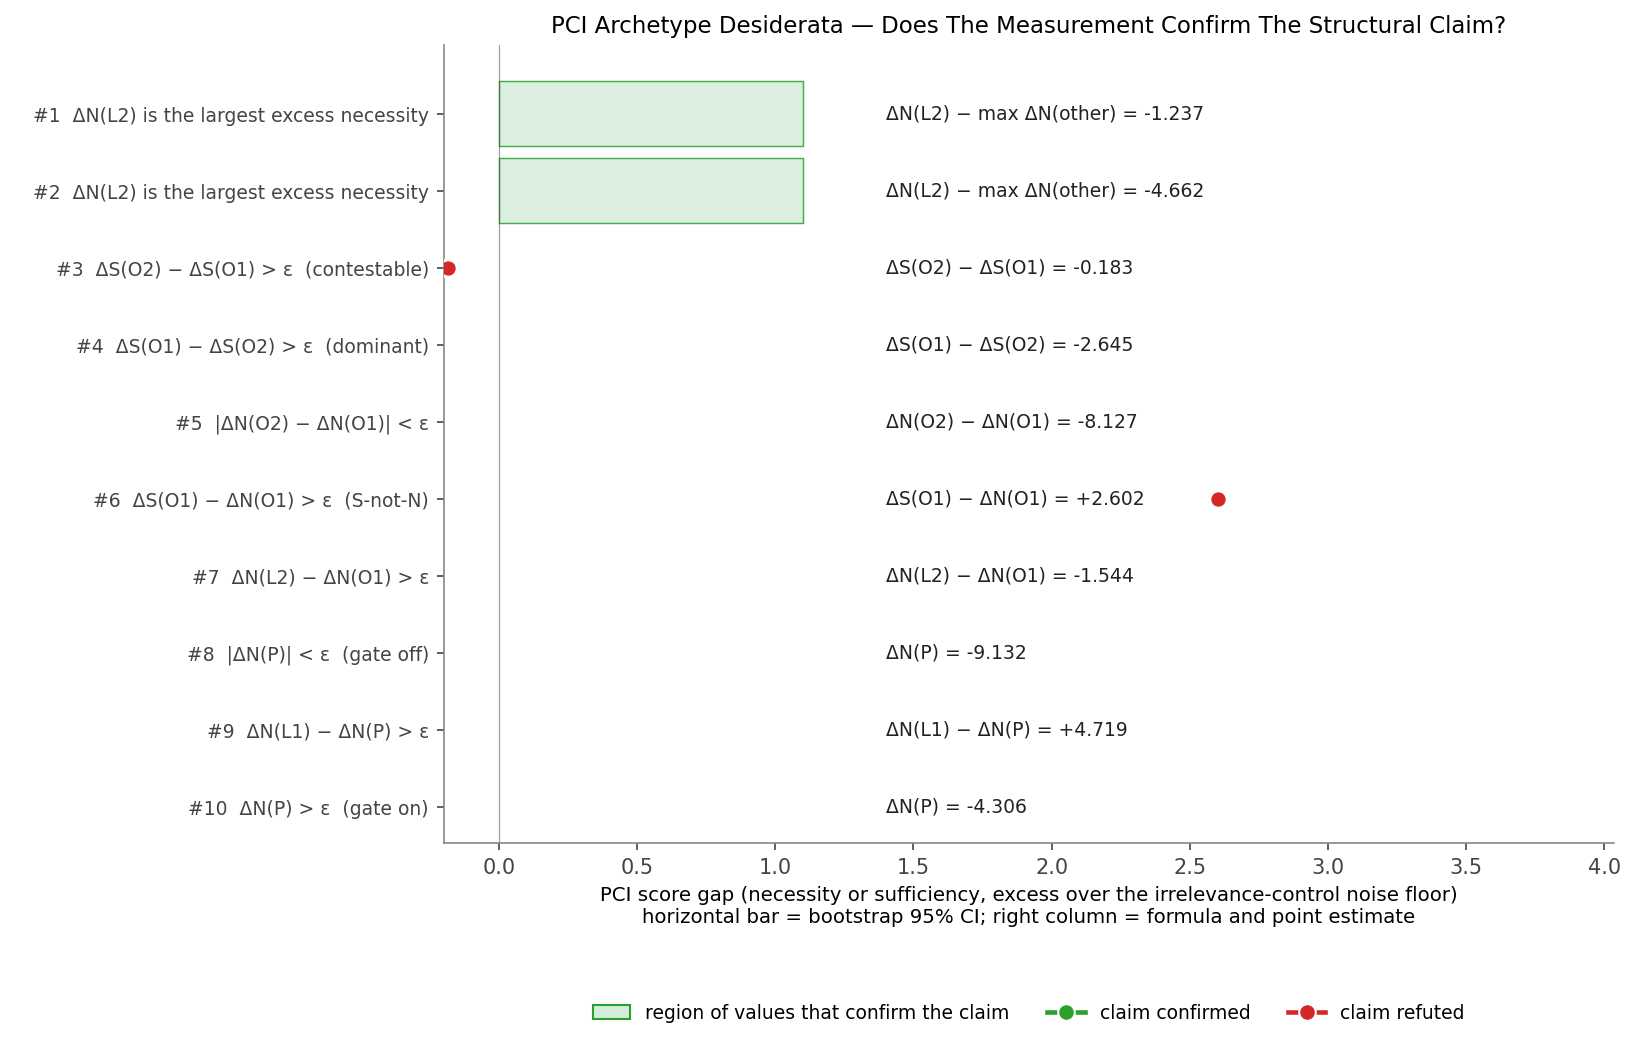
\includegraphics[width=0.92\linewidth]{figures/archetypes_threshold_forest.png}
\caption{\textbf{\ourapproach recovers the actual-causality verdicts on a
four-archetype synthetic model.} Each row is one archetype desideratum (linear
necessity/sufficiency, overdetermination, preemption, irrelevance control); the
dot is the bootstrap point estimate of the relevant $\Delta$ score, the bar its
$95\%$ CI, and the green band the pass region given the data-derived threshold
$\epsilon \approx 0.151$. All ten dots fall inside their bands. Full model,
estimator, and per-row analysis in Appendix~\ref{sub:synthetic}.}
\label{fig:eval_archetypes}
\end{figure}

\subsection{SHAP and Causal SHAP}
\label{sec:eval_shap}
\ourapproach separates direct and indirect causal contributions; SHAP-based
attribution collapses them into one number. Both plain and Causal SHAP decompose a prediction's departure
from a population mean. Because that mean is not the realized outcome, this choice
produces two failures at once. First, they assign attribution backward, against the
arrows of the causal graph; Causal SHAP's interventional correction fixes only part
of this. Second, they tie together the direct and indirect causes of an outcome
that a context-sensitive method should keep separate. \ourapproach{}'s
realized-outcome reference and witness mechanism fix both problems, separating the
direct cause from the indirect one at every instance, as
Table~\ref{tab:eval_shap_desiderata} summarizes on the signal-with-mediation
example ($X \to M \to Y$).

\begin{table}[htbp]
\centering
\small
\begin{tabular}{lccc}
\toprule
Desideratum & Plain SHAP & Causal SHAP & \ourapproach \\
\midrule
D-XY: $X$ genuinely causes $Y$ & \checkmark & \checkmark & \checkmark \\
D-MY: $M$ genuinely causes $Y$ & \checkmark & \checkmark & \checkmark \\
D-XM: $X$ genuinely causes $M$ & \checkmark & \checkmark & \checkmark \\
D-YX: no backward attribution from $Y$ to $X$ & \texttimes & \checkmark & \checkmark \\
D-YM: no backward attribution from $Y$ to $M$ & \texttimes & \texttimes & \checkmark \\
D-MX: no backward attribution from $M$ to $X$ & \texttimes & \texttimes & \checkmark \\
D-MXY: the direct cause $M$ outranks the indirect cause $X$ & \texttimes & \texttimes & \checkmark \\
\bottomrule
\end{tabular}
\caption{Desiderata satisfied (\checkmark) or violated (\texttimes) by plain SHAP,
Causal SHAP, and \ourapproach on the signal-with-mediation example. Causal SHAP's
interventional correction repairs only D-YX. Full numeric values and witness-set
variants in Table~\ref{tab:signal_desid}.}
\label{tab:eval_shap_desiderata}
\end{table}

Section~\ref{sec:shap_examples}
states these failures as formal desiderata and works through both in full on two worked
examples (OBCB and the signal-with-mediation chain), with the formal SHAP and Causal
SHAP definitions in Appendix~\ref{app:signal}.

\subsection{The Differential Causal Effect}
\label{sec:eval_dce}
The next comparison targets a causal-effect attribution method: the
Differential Causal Effect (DCE) attributes an outcome change to features via local
derivatives of the structural map. On a model with a non-monotone internal response,
DCE and \ourapproach can disagree on sign and magnitude where the local gradient is
unrepresentative of the counterfactual contrast \ourapproach integrates over:
tracking the realized-outcome contrast keeps
\ourapproach's attribution aligned with each feature's structural role, without
depending on a single local derivative.

\begin{figure}[htbp]
\centering
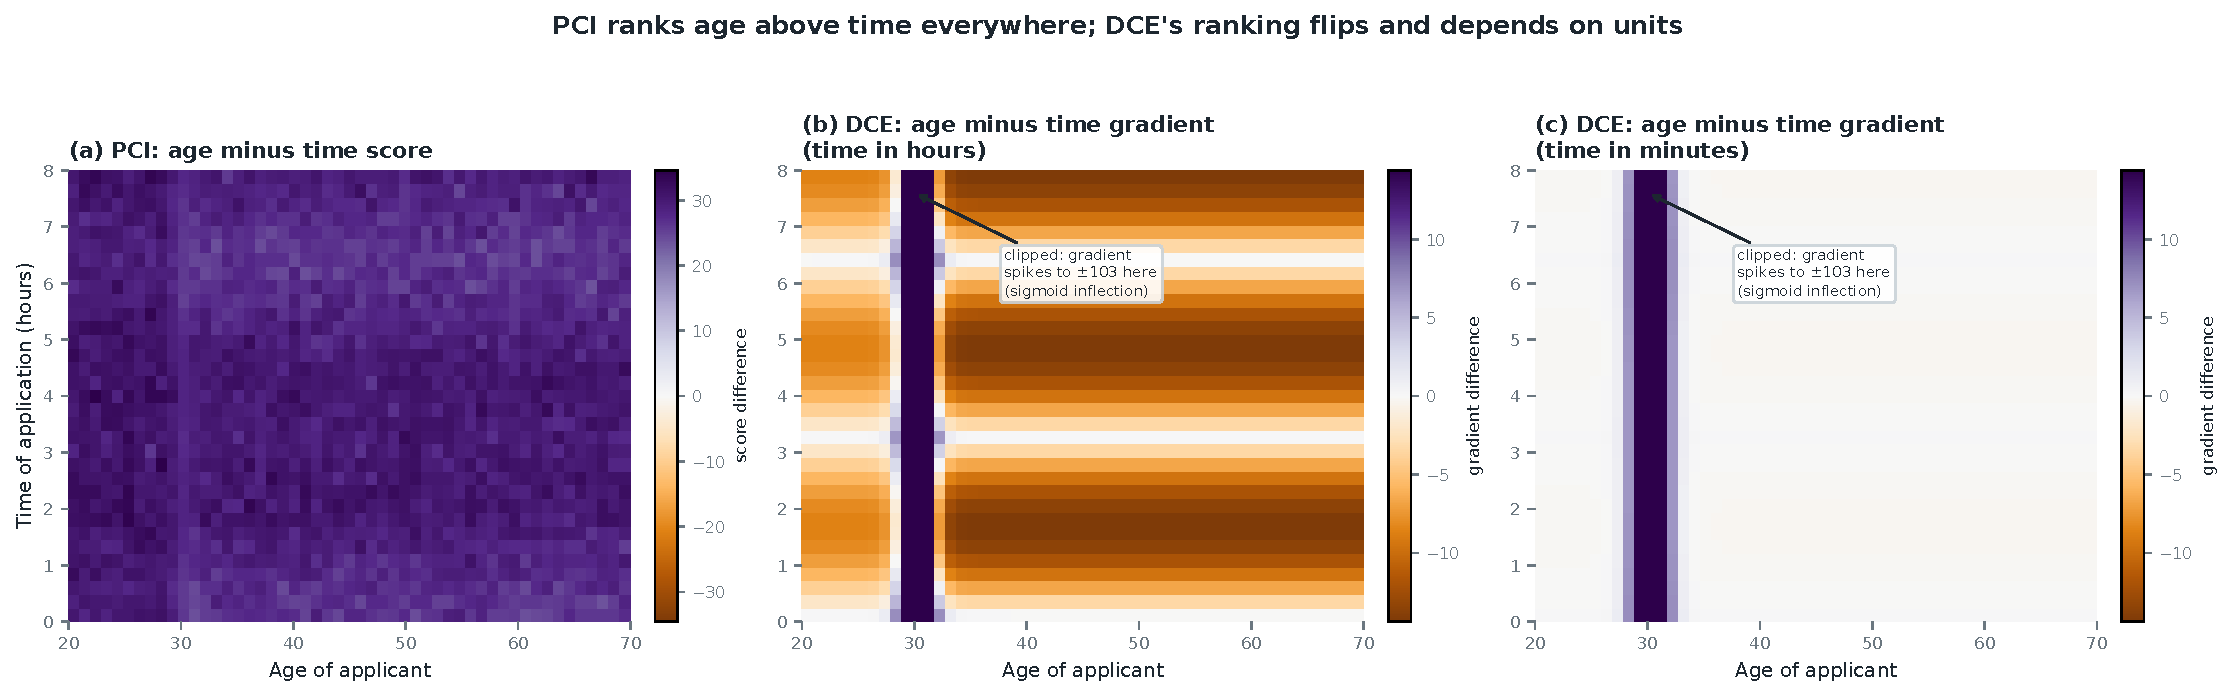
\includegraphics[width=\linewidth]{figures/dce_contrast_overview.pdf}
\caption{\textbf{\ourapproach stays consistent where DCE does not.} \textbf{(a)}
\ourapproach ranks age above time of application everywhere on the credit-limit
grid; the gap is somewhat denser around the age of rapid change (the sigmoid's
steep region) but stays positive throughout. \textbf{(b), (c)} The same contrast for DCE, on the hours and minutes
time scales: DCE favours time of application over most of the grid (the
opposite of \ourapproach's verdict), except in a narrow band where its
gradient spikes at the sigmoid's inflection point, and that pattern itself
depends on which time unit is used. Full discussion in Appendix~\ref{sec:DCE}.}
\label{fig:eval_dce}
\end{figure}

Appendix~\ref{sec:DCE} shows the full contrast over a credit-limit grid.

\subsection{Scaling past exact actual causality}
\label{sec:eval_scaling}
Actual-cause computation requires enumerating counterfactual subsets, which
is exponential; \ourapproach replaces enumeration with a Monte Carlo thin search.
On a controlled family of problems (Appendix~\ref{sec:ac_benchmark}), exact subset
enumeration times out at about $17$ variables, whereas the necessity-only
\ourapproach estimator continues to roughly $73$--$145$ variables under an
undemanding sample budget and a per-size compute cap of $60$ minutes. It sustains a
correct-attribution rate above $0.85$ up to about $60$ variables while visiting
several orders of magnitude fewer cause--witness configurations.

\begin{figure}[htbp]
\centering
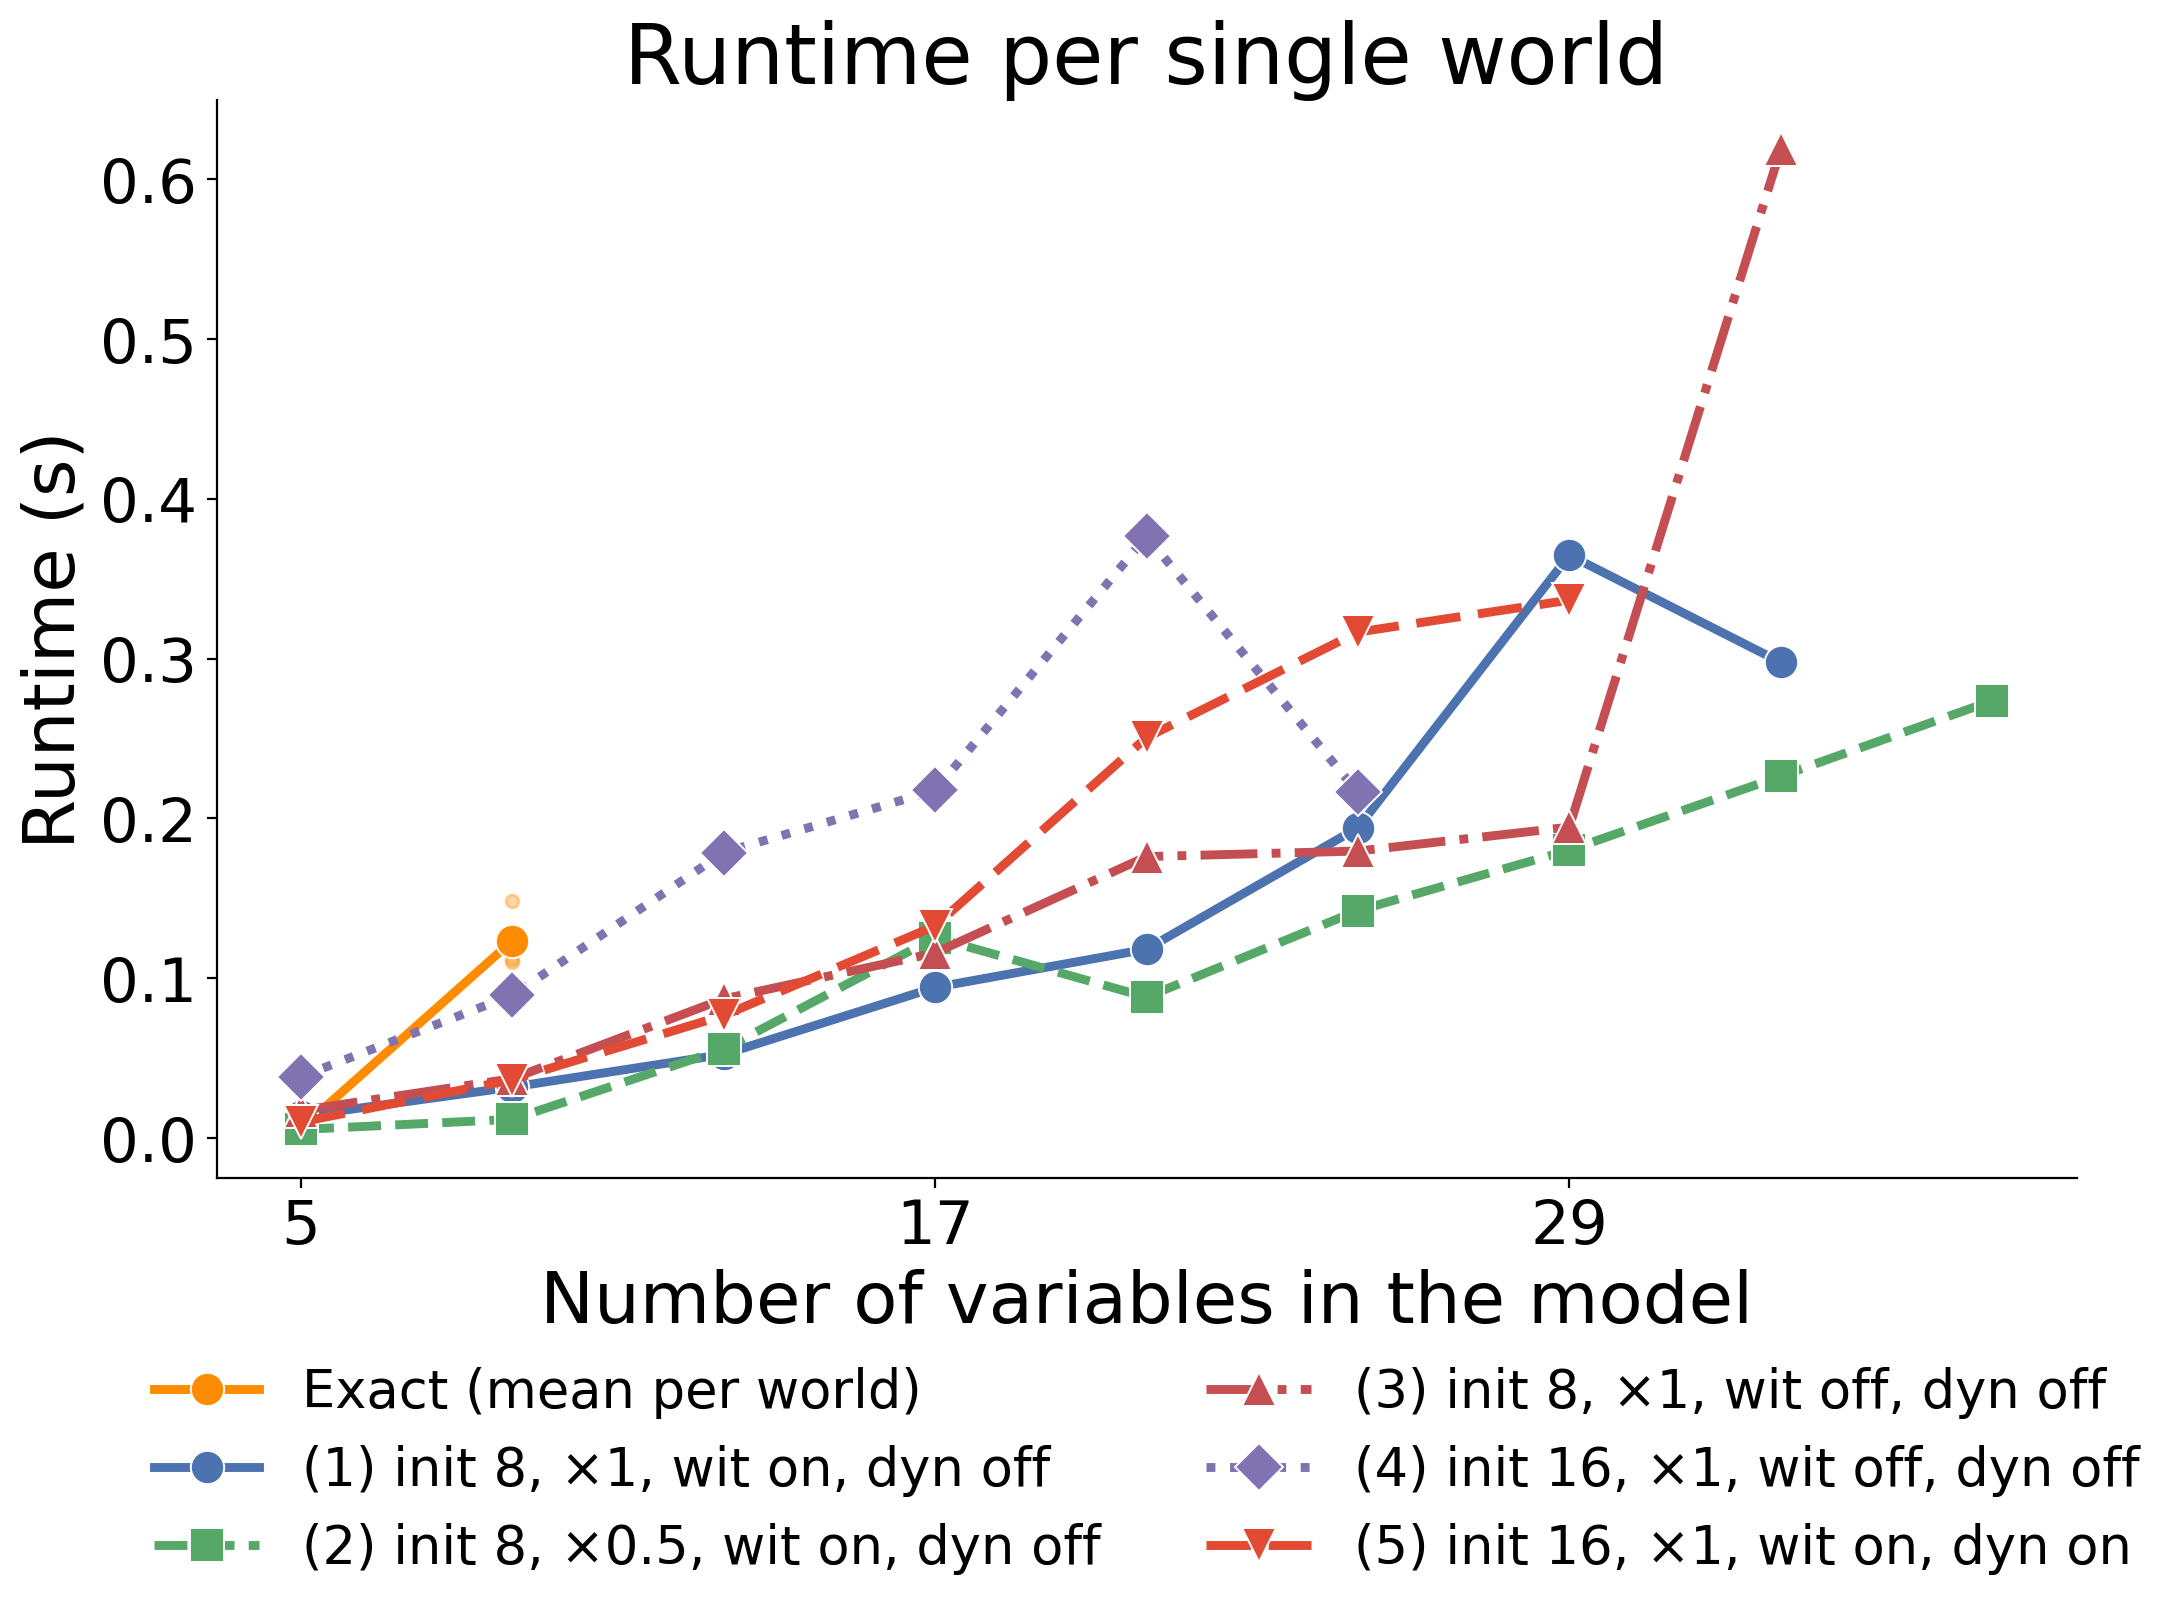
\includegraphics[width=0.49\linewidth]{docs/source/ac_benchmark/plot1_runtime.png}
\hfill
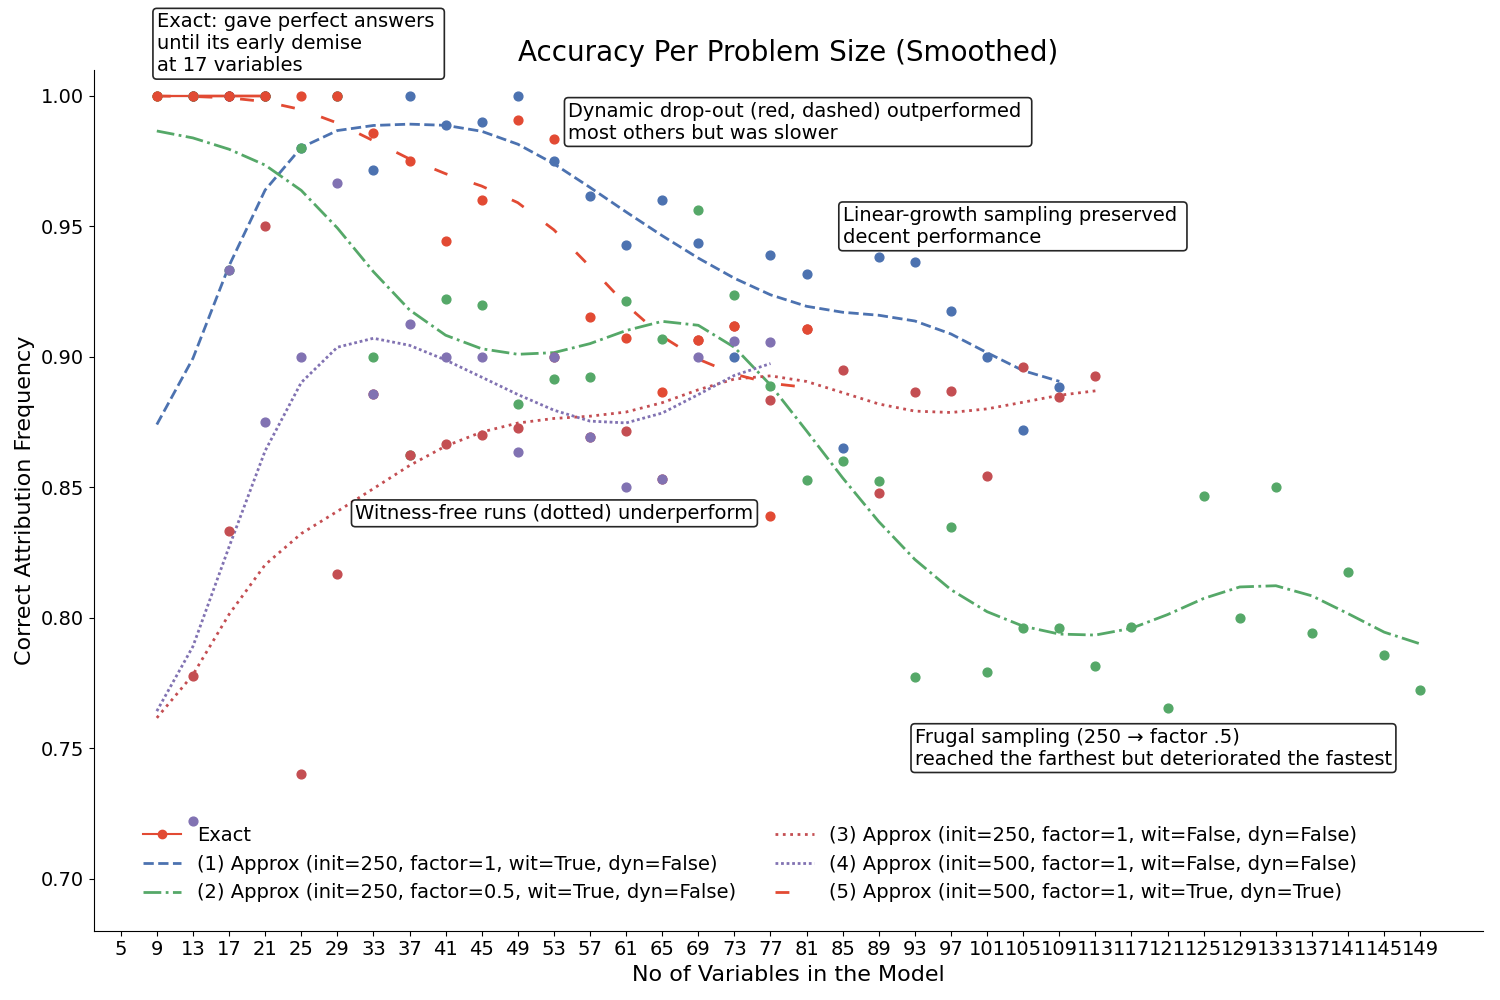
\includegraphics[width=0.49\linewidth]{docs/source/ac_benchmark/plot3_accuracy.png}
\caption{\textbf{\ourapproach's estimator continues to work well past the point
where exact actual-cause enumeration gives out.} Left, wall-clock vs.\ problem
size: exact subset enumeration times out near $17$ variables, while the
\ourapproach estimator continues to roughly $73$--$145$. Right,
correct-attribution rate: witness-enabled configurations stay above
$0.85$ well past the exact cut-off, degrading gradually with problem size. Full
benchmark protocol in Appendix~\ref{sec:ac_benchmark}.}
\label{fig:eval_scaling}
\end{figure}

\subsection{Continuous, dynamical outcomes}
\label{sec:eval_sir}
Actual causality has a second limit besides scale: it offers no verdict when the
outcome is continuous and the causes interact through a dynamical system. On a
Bayesian SIR (susceptible--infected--recovered) model with two non-pharmaceutical
policies and a threshold (peak-overshoot) outcome (Appendix~\ref{sec:sir_benchmark}),
but-for analysis cannot separate the two policies; \ourapproach assigns
lockdown roughly twice the responsibility of masking, with the gap driven by the
necessity term under witness pinning. Unlike the archetype benchmark above, this
is a single-run point estimate: we do not yet report a confidence interval
across seeds here.

\begin{figure}[htbp]
\centering
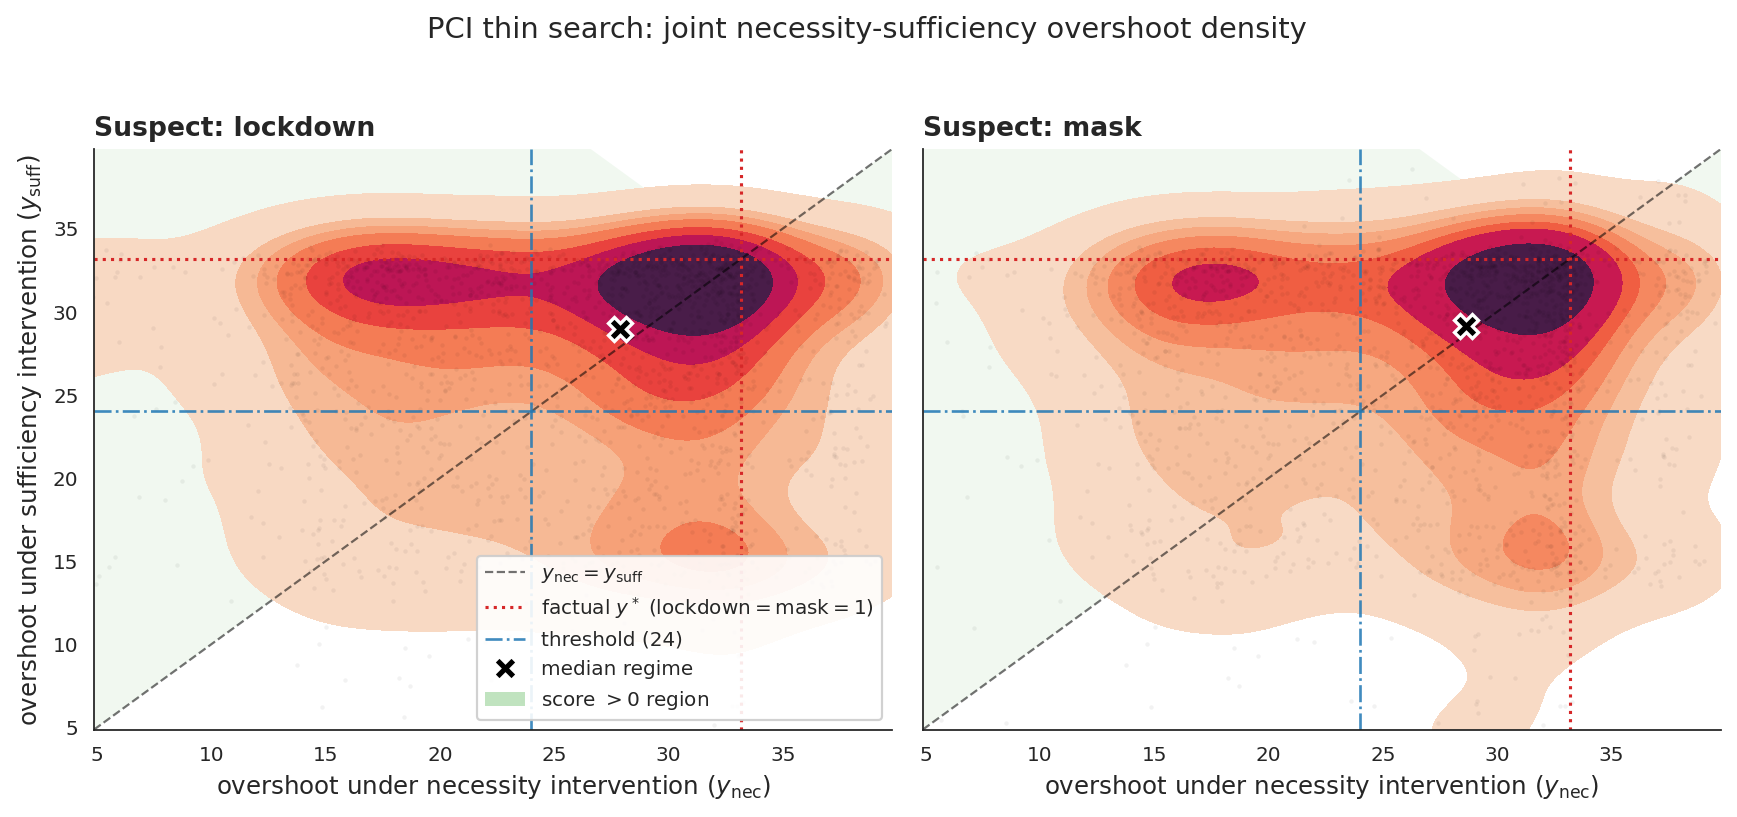
\includegraphics[width=0.80\linewidth]{docs/source/sir_benchmark/sir_heatmap.png}
\caption{\textbf{\ourapproach separates interacting policies on a continuous
dynamical outcome.} Joint necessity-sufficiency over the two policies for the
peak-overshoot event; lockdown carries roughly twice the responsibility of masking
where but-for analysis ties them. Full model and query in
Appendix~\ref{sec:sir_benchmark}.}
\label{fig:eval_sir}
\end{figure}

\subsection{A real-world deployed model}
\label{sec:eval_avm}
Finally, \ourapproach runs on a deployed automated valuation model (AVM) with
machine-learned components trained on millions of points, a regime where actual
causality is intractable and SHAP is the practical default
(Appendix~\ref{sec:avm}). \ourapproach returns a structured, context-sensitive
attribution across the model's internal variables; SHAP, by contrast, concentrates
almost all responsibility on a few downstream variables and places little weight
on the rest. This deployed model has no independently known ground truth.
\ourapproach and SHAP disagree here in the same qualitative direction already
validated by the synthetic benchmark's ground truth, but on its own the AVM
case demonstrates feasibility; it does not independently confirm correctness
(\cref{sec:discussion}).

\begin{figure}[htbp]
\centering
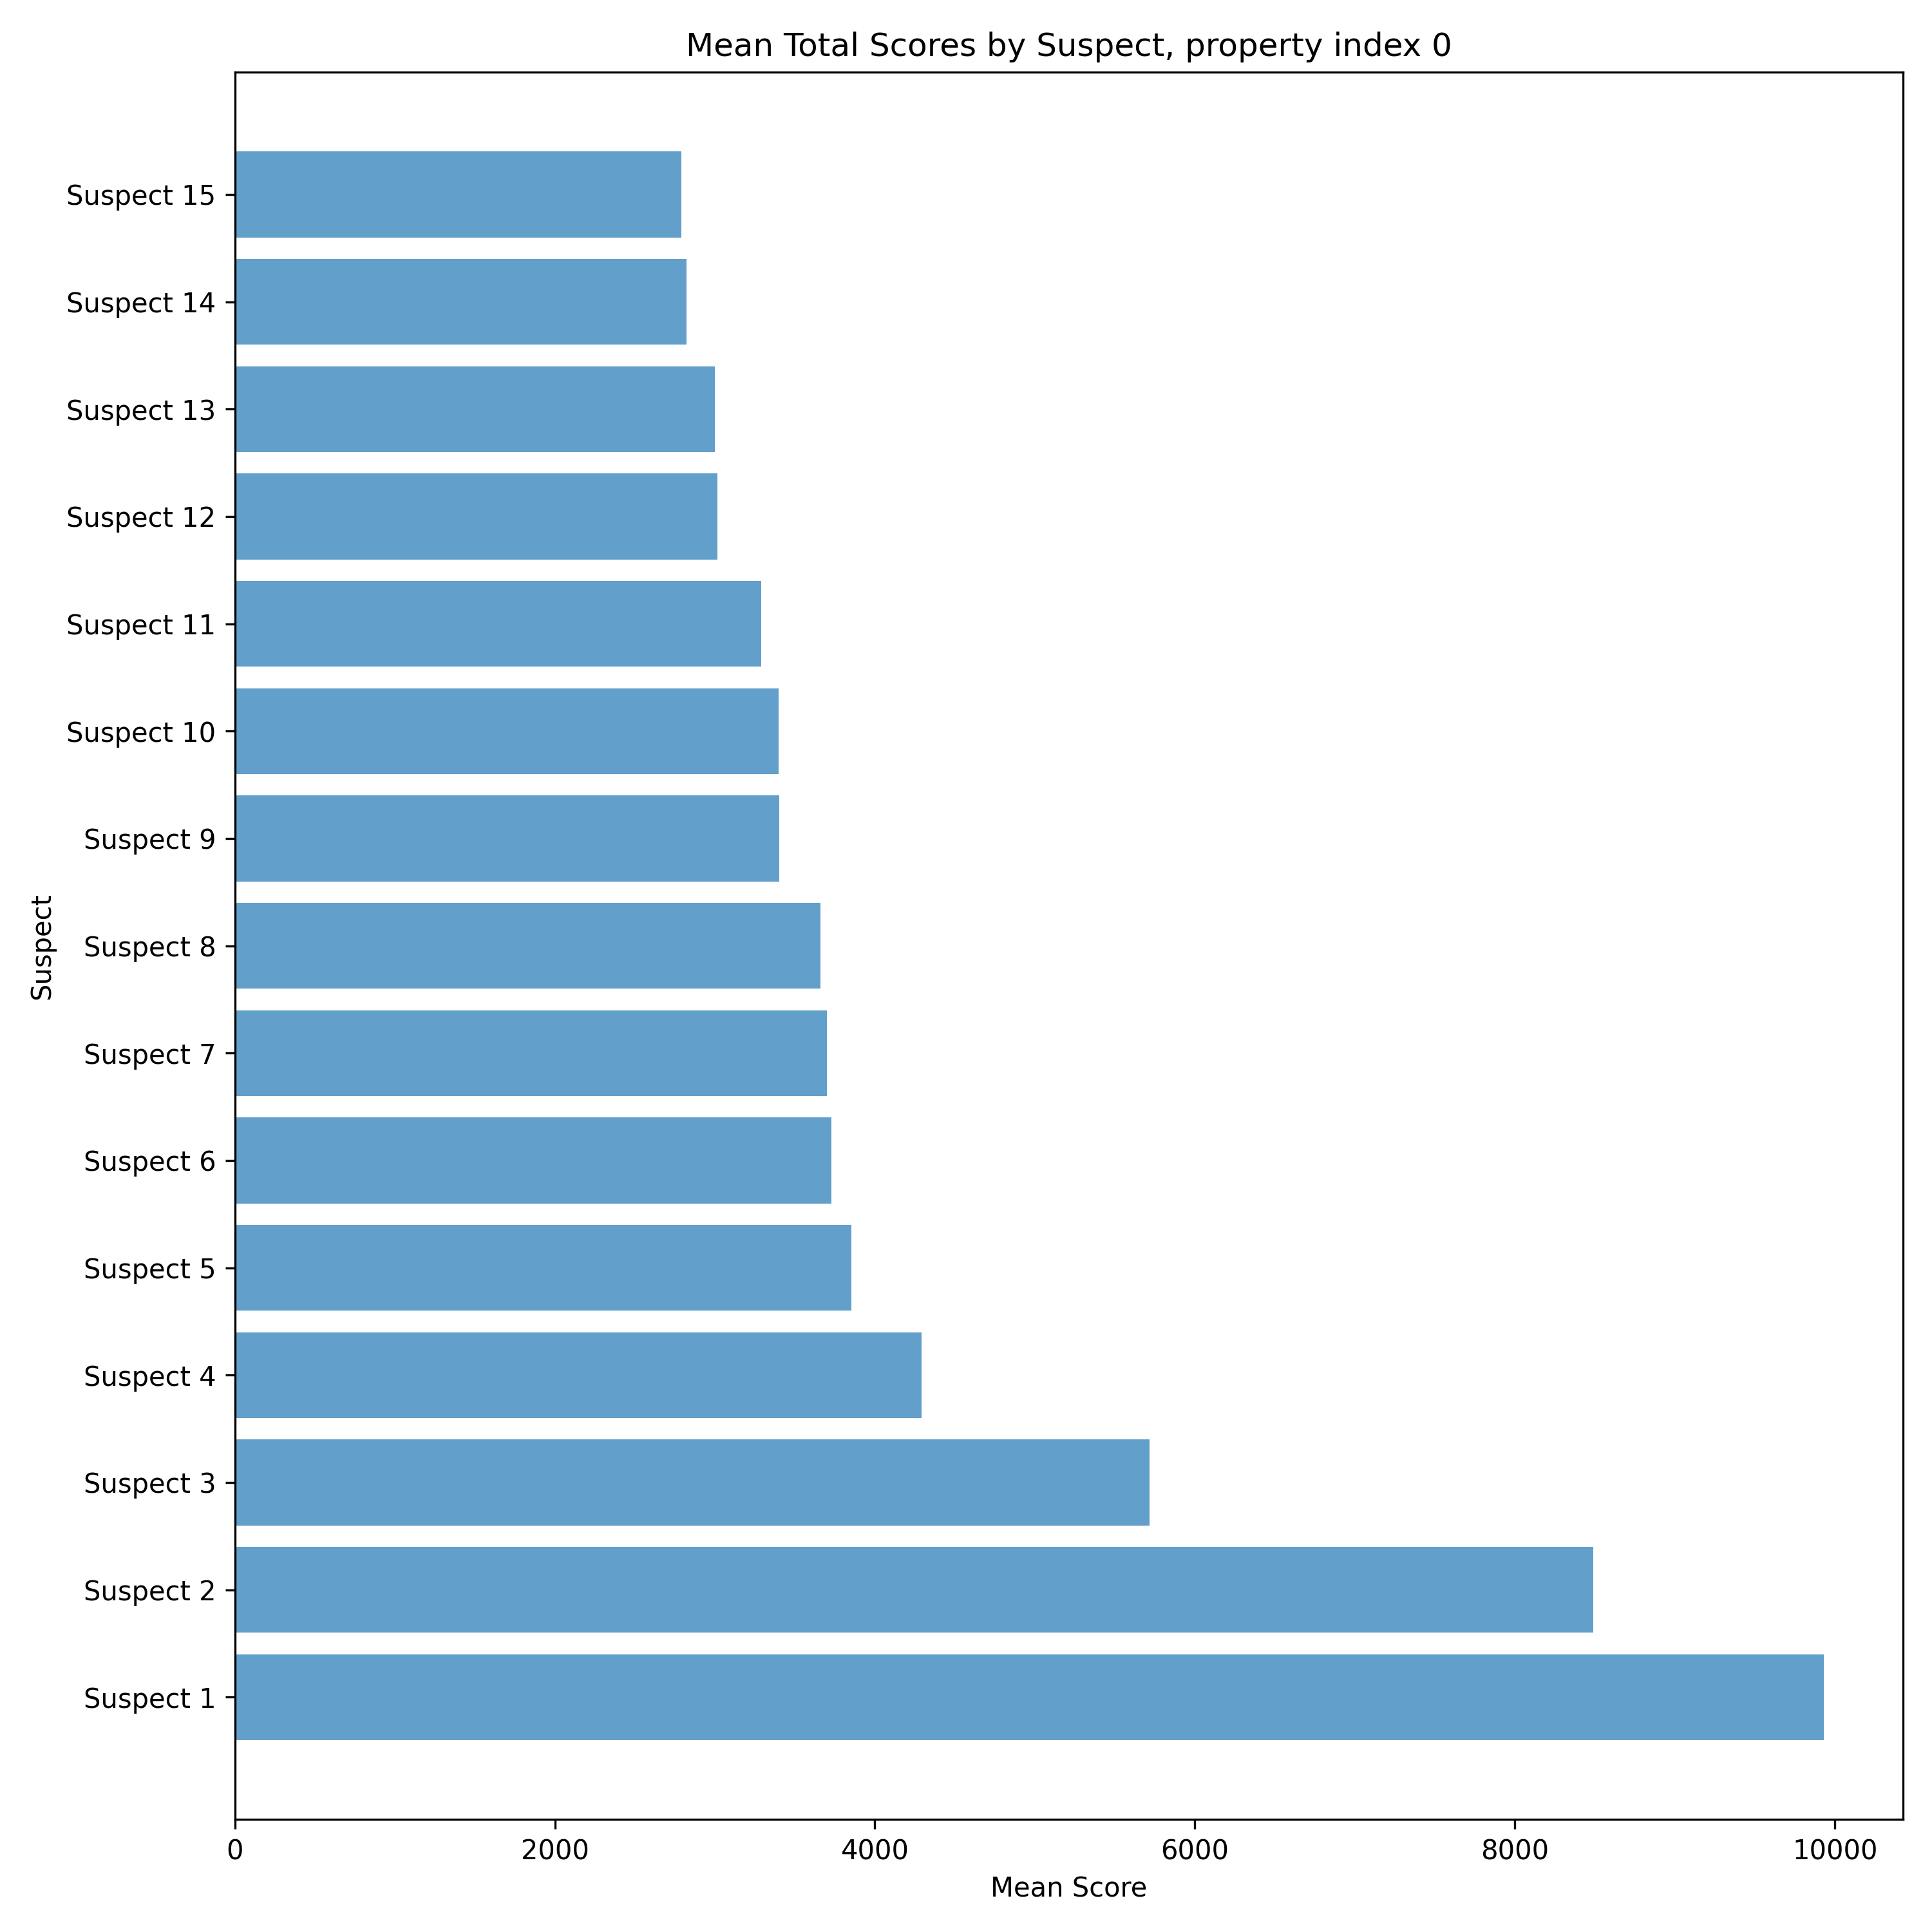
\includegraphics[width=0.49\linewidth]{figures/search_query_figure.png}
\hfill
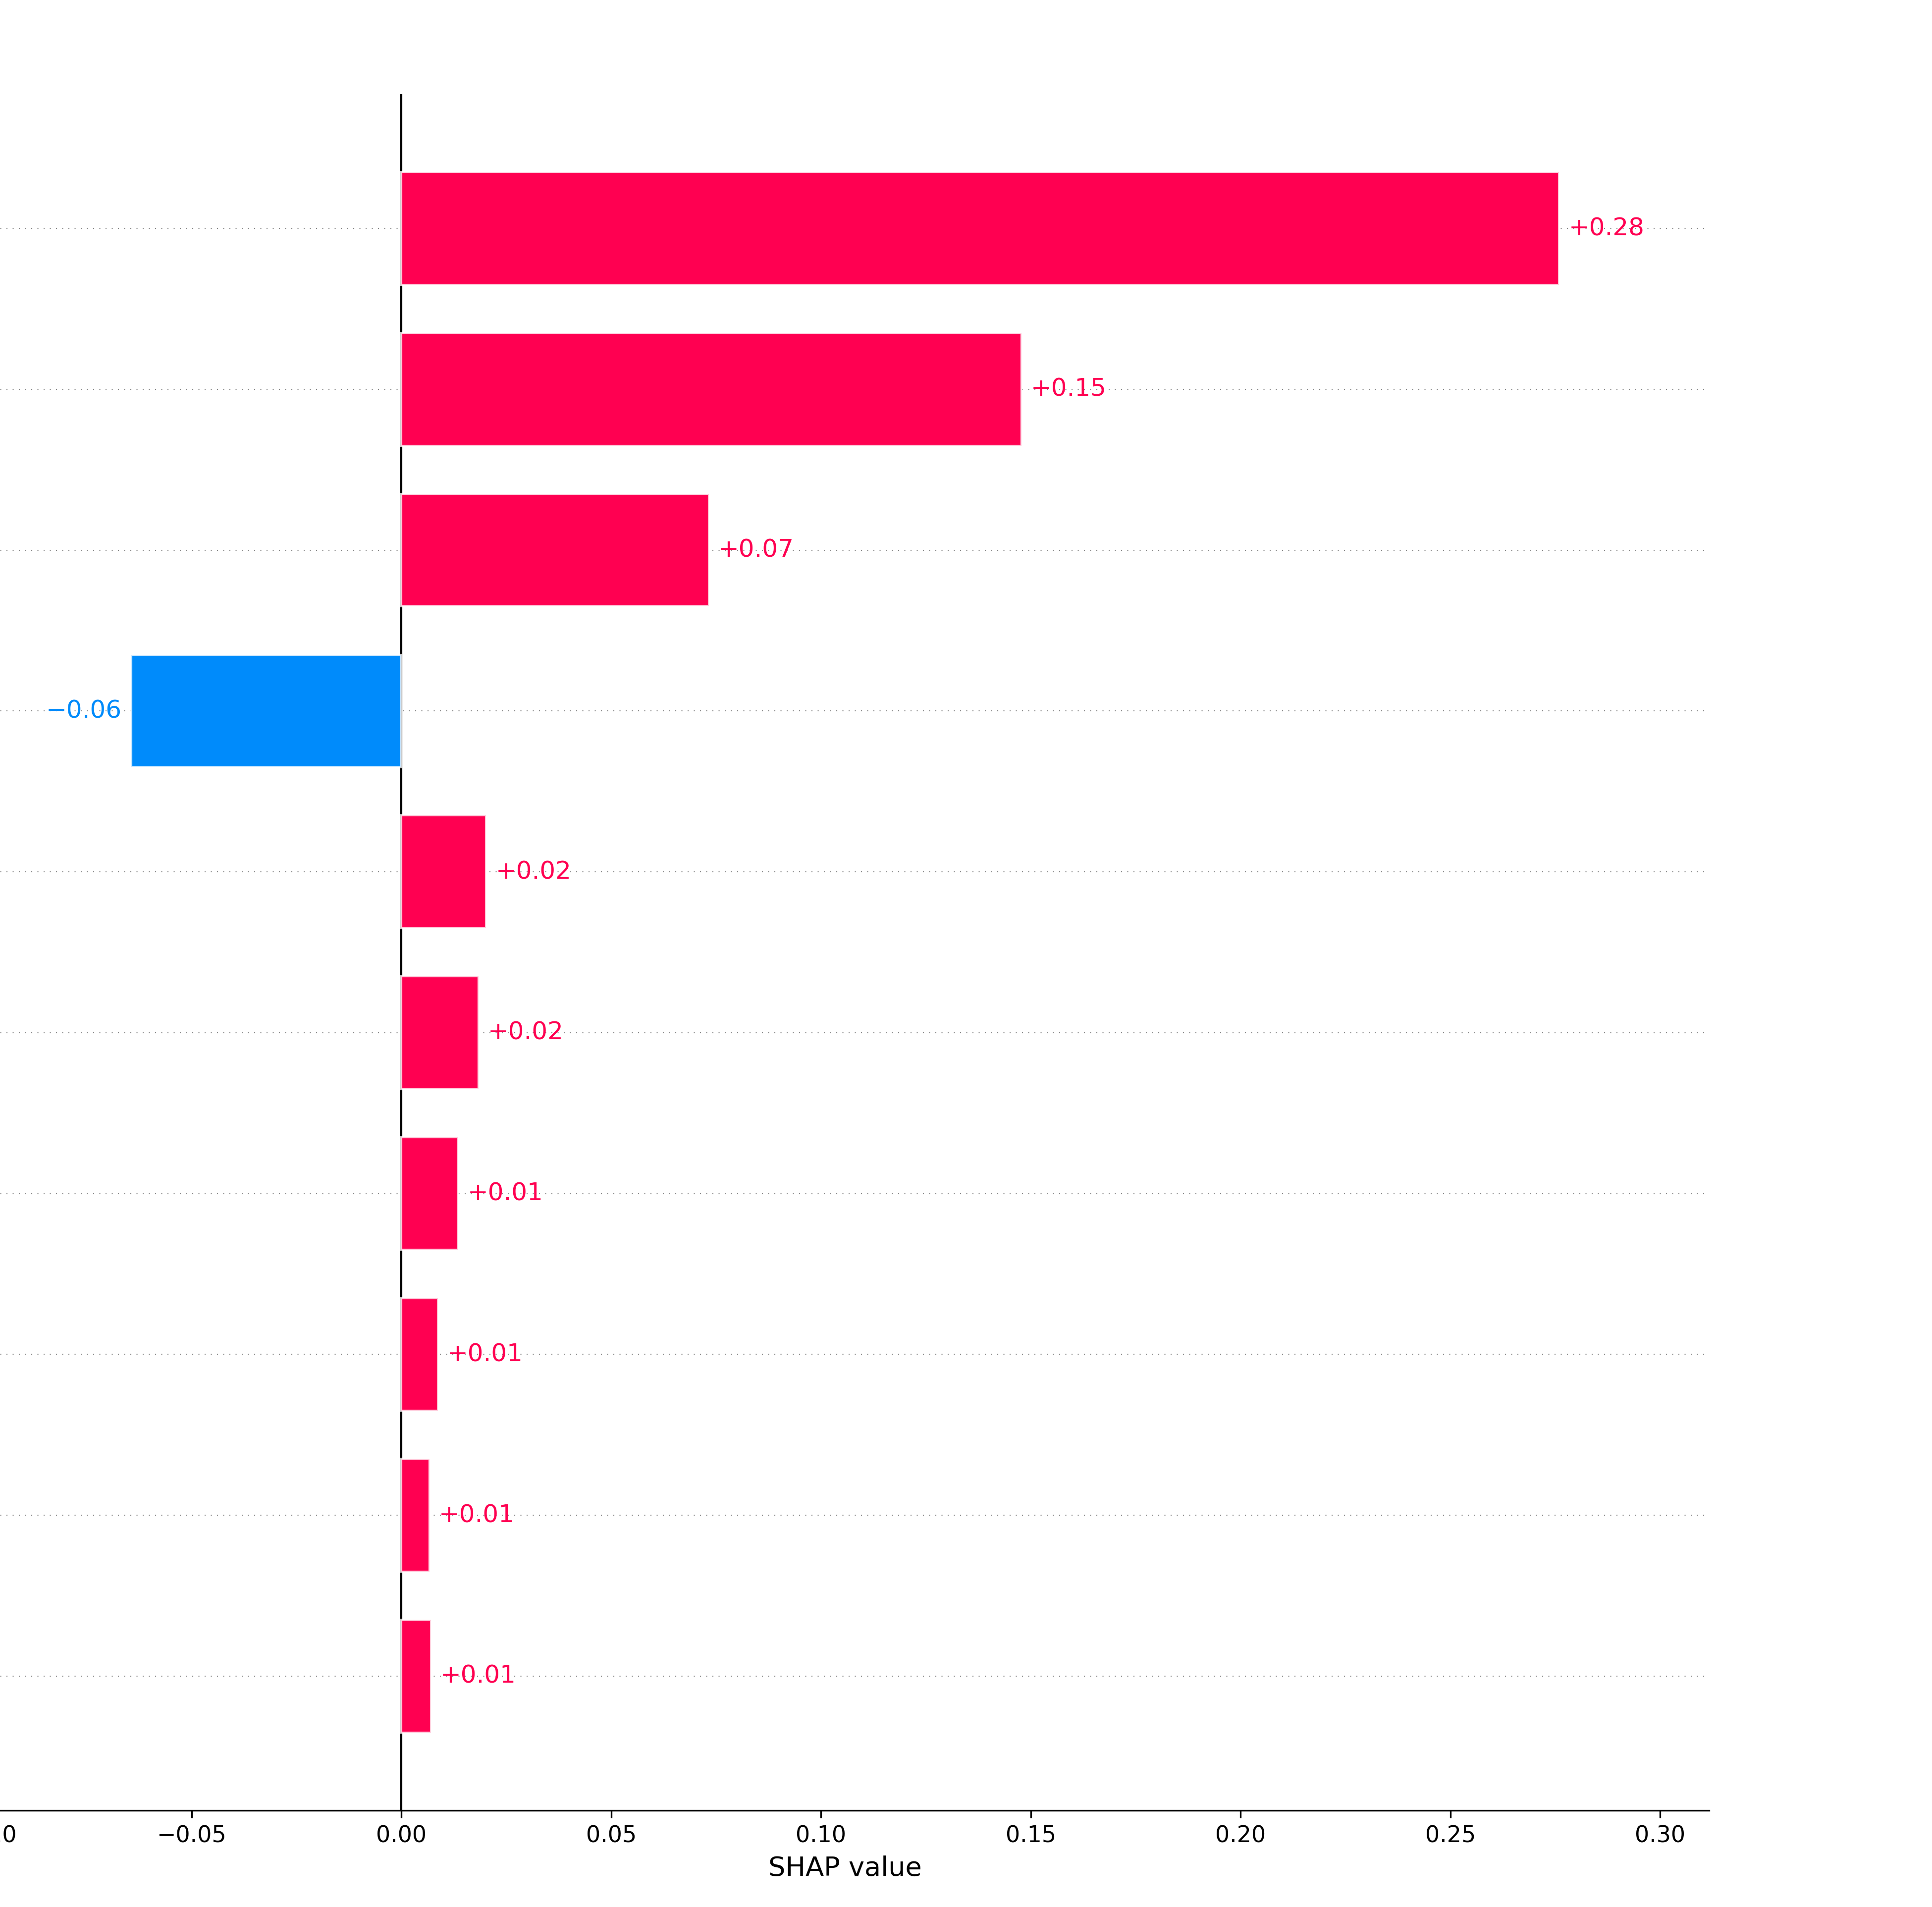
\includegraphics[width=0.49\linewidth]{figures/shap_figure.png}
\caption{\textbf{\ourapproach vs.\ SHAP on a deployed automated valuation model.}
Both panels show a selection of the model's internal variables; real variable
names are withheld under an NDA with the model's operator, and the two panels
rank their own top variables independently, so a given position in one panel
does not correspond to the same variable in the other. Left: \ourapproach's
context-sensitive attribution across the AVM's internal variables. Right: SHAP
concentrates responsibility on a few downstream variables. Full pipeline and
anonymized structure in Appendix~\ref{sec:avm}.}
\label{fig:eval_avm}
\end{figure}

\medskip\noindent Across these settings \ourapproach matches actual-causality verdicts on canonical archetypes and extends past them where they do not apply, at a cost that remains tractable; the full protocols, derivations, and additional figures are collected in Appendices~\ref{app:obcb}--\ref{sec:avm}. Sections~\ref{sec:shap_examples}--\ref{sub:pearl_actual_cause_prob} develop these comparative claims in full before \cref{sec:discussion} draws out the implications.
